\epigraph{\emph{
  ``An algorithm must be seen to be believed.''
}}{ Donald Knuth }

In this section, we evaluate some strategies for clustering. At first, we will show, how a single day of news events are clustered. Given the timeframe of this thesis, it was not possible to elaborately test multiple days clustering. It is a notoriously difficult topic that greatly relies on the data and time. Originally it was intended to use a scraped data set over several month, categorized by date, with as much meta data as possible. As this is at the barrier of legality, a smaller standardized data set, namely the BBC data set by \cite{BBCData2006} was used. In the original data set, it was possible to assume that the data was ordered and sorted by day. Several thousand articles could then be easily clustered on a daily basis and enhanced over the course of several months. Instead, we are focusing on how the BBC data set can be clustered and evaluated. Multiple day clustering will be depicted, but not in any form evaluated.\\

The BBC data set had a few limitations in the sense that dates and meta data were not provided. As such we treat the data as a a bulk of events occurring in the time frame of 2004-2005. Fortunately unlike real world data the articles are tagged with precise categorical labels, so external evaluation measures were an option. There were limitations in time to find a more adequate set of articles that were consecutively sorted by day in a broader category such as ``world news''.\\

The clustering was done in several steps, similar to the Columbia Newsblaster system.\cite{NewsBlaster2002} A hierarchical clustering approach by first clustering events into categories like politics, business or entertainment and second clustering the categories into distinct events. The classification in the first step guarantees some broader topical cohesion. In the BBC data set a purity of up to 94\% could be achieved on the test set. This is unusually high, but is probably due to the normalized data set, that represents the classes exceptionally well. The real world data set could go as high as 45\% purity and less. The purity on the BBC data set varies broadly between 79\% and 94\%. This variability results in overlapping topics, where the majority of documents in a cluster are in the same class. Each of the resulting clusters resembling the underlying classes are re clustered. In this second step, clusters represent news events on several topics per cluster.\\

Some final words on the measurement of the two steps. In the first step, it is easy to evaluate how well documents were assigned to their respective classes. In the second step however, evaluation is not that simple. At this point, we are interested in document similarity based on content and not class labels. The results of the second clustering are informal and not measured.

\section{Single day clustering}

Single day clustering is done by focusing on one specific date. The hypothesis is, as long as there are no major news headlines, documents will have a high variance in vector space. Thus, there will be more clusters. Major news headlines absorb almost all articles into single clusters. That is expected, as news are often homogeneous in their topic selection. In the original data set were clusters, that absorbed roughly 90\% of the articles, in case of terrorist attacks or huge world wide events. The problem arises, that articles not covering the event, were clustered into that one cluster monolith as well.\\

In the following the two steps are refined. First we want to classify news events by classes, in case of the BBC data set: politics, business, entertainment, tech and sports. For this it is possible to use algorithms with a hard number of final clusters, to classify documents into the classes. Alternatively one could use a supervised classifier, which in practice, is much more accurate. See \cite{LearningMultiLabelKmeans2013} for a real world example learning labels in comparison of \kmeans{} and a \emph{supervised classifier}. Second, the resulting clusters, now assigned by news category, are clustered again. This time, the clustering algorithm has the constraint of automatically detecting the cluster numbers. For this a hierarchical algorithm with soft thresholds was chosen e.g. BIRCH and Ward linkage. The resulting clusters resemble news events, dealing with a similar topic. 

\section{Implementation}
The implementation of a more general clustering algorithm in the text domain can vary drastically. A general scheme is given by algorithm \ref{general_clustering}.

  \begin{algorithm}[H]
  \begin{algorithmic}[1]
    \caption{General clustering}\label{general_clustering}
    \Function{general\_cluster}{$X_{train},y_{train},\kappa,\alpha,d$}
      \State $X_{norm},y_{norm} = normalize_{text}(X_{train},y_{train})$
      \State $X_{project},y_{project} = project(X_{norm},y_{norm})$
      \State $X_{trans},y_{trans} = transform(X_{project},y_{project})$

      \State $X_{lsi} = lsa(X_{trans}, topics=\alpha)$
      \State $X_{dim} = reduce\_dimensions(X_{lsi}, dimensions=d)$
      \State $X_{sim} = similarity(X_{dim})$
      \State $X_{scaled} = scale(X_{sim})$
      \State $model,centroids,labels,k = cluster(X_{scaled}, clusters=\kappa)$

      \State \Return $model,centroids,labels,k$
    \EndFunction
  \end{algorithmic}
  \end{algorithm}

The general implementation \ref{general_clustering} is separated into several steps. As input, the function gets a training set $X_{train}$ and a label set $y_{train}$. $\kappa$ is an optional parameter for the total amount of cluster centers. $\alpha$ a parameter that sets a desired size of topics for models like \lsa{}. And a dimension $d$ to reduce $X$ to, for visualization purposes by e.g. \pca{}. In general we assume that the data $X_{train}$ is of any textual sort, the preprocessing needs to do the necessary steps that fits the function. Moreover it is of utmost importance to think in terms of vectorized code. Any procedures gradually transform a document into the vector space. After this all rules by linear algebra hold.

  \begin{enumerate}
    \item \emph{normalize} takes $X_{train}$ and $y_{train}$ to remove special characters, stop words, numbers. Lower casing any words and removing non English characters or sentences. 
    \item \emph{project} is any kind of projection strategy via \wordnet{}, noun phrases or named entities, lowering word sense disambiguation and dimensions. This step deals with the initial seed of knowledge that is used throughout the algorithm.
    \item \emph{transform} takes in the projected data and transforms it via \tfidf{}, word pruning, as well as ngram enhancement.
    \item \emph{lsa} is an optional step that transforms the resulting data to dense low dimensional matrices, keeping as much variance as possible while reducing noise. In this case \lsa{} was used but \lda{} or \hdp{} would be an option as well. 
    \item \emph{reduce\_dimensions} is an alternative step that reduces the dimension of the data to 2d or 3d plotting clusters. This is typically done by \pca{}.
    \item \emph{similarity} transforms document x term vectors to document to document similarity by cosine or euclidean distance measures.
    \item \emph{scale} is a second normalization step, scaling the data by variance and average.
    \item \emph{cluster} finally takes the matrix $X_{scaled}$ and clusters based on a hard constrained clustering number. If not supplied the clustering algorithm needs to predict a cluster number automatically. This results in the actual cluster amount $k$. The resulting trained clustering $model$. The $centroids$ in case they are actively calculated e.g. by \kmeans{}. And finally the $labels$, the assignment from a document to a corresponding cluster.
  \end{enumerate}

The implementation is a rough sketch of a real clustering scheme. In reality most of the before mentioned steps can be parameterized or constrained by additional arguments. Either a configuration object is specified or an extensive API used to create clustering scripts. The API used was $scikit-learn$ by \cite{ScikitLearn} and is part of the huge scientific computing libraries written in Python, such as $numpy$, $scipy$, $pandas$ etc. From this, we can generalize a clustering scheme for a single day.

  \begin{algorithm}[H]
  \begin{algorithmic}[1]
    \caption{Single day clustering}\label{single_day_clustering}
      \State $X_{train},y_{train} = get\_data(timestamp)$
      \State $model,centroids,labels,k = general\_cluster(X_{train},y_{train},\kappa,\alpha)$
      \State $X_{assigned} = get\_assigned\_documents(X_{train},labels)$
      \State $news\_labels = []$
      \For{$c \in X_{assigned}$}
        \State $model',centroids',labels',k' = general\_cluster(c,nil,\alpha)$
        \State $assign(news\_labels, X_{train}, labels')$
      \EndFor
      \State \Return $news\_labels$
  \end{algorithmic}
  \end{algorithm}

The implementation \ref{single_day_clustering} is a rough sketch of what the \emph{News-Clusty} system does. First, get the data by a timestamp e.g. ``20150701'', cluster the data by a fixed $\kappa$ and then use the resulting cluster assignments $X_{assigned}$ to group news events. Note that $general\_cluster$ in the second run has a $nil$ argument, because we do not want to constrain by cluster amount. The clustering now depends entirely on the variation of the intermediate procedures of $general\_cluster$ and is now an optimization problem. 

\section{Evaluation}
In the evaluation section, the before mentioned measuring strategies are used. Several different strategies are weighted against each other. It was found, that there are several different ways with a good performance in the categorical clustering approach. The second clustering is not of utmost importance in the evaluation and depicted later. A major problem is, that several parts of the proposed algorithm, rely on parameter estimation. To narrow down this combinatoric explosion of parameters, several assumptions can be made.

  \begin{enumerate}
    \item Limiting the strategies to simple word tokens and their document titles except stop words, noun phrases and NER tags as well as \wordnet{} first hypernym and \wordnet{} lemmatization.

    \item \emph{Transforming} by \tfidf{} with a 80\% maximum threshold and a hard count $3$ for minimum threshold, excluding ngrams.

    \item \emph{topic modeling}, whether \lsa{} or \lda{} should be used or not. The topic size is manually adjusted.

    \item Setting the \emph{distance measure} to \emph{cosine}.

    \item \emph{clustering algorithm} constrains, such as density thresholds and maximum \emph{HAC} depths. Classification is constrained by $k=5$ for the categories of the BBC data set.
  \end{enumerate}

A comparison of the different strategies with \lsa{} enabled, for the classification task, is shown in table \ref{comparison_single_with_lsa}. Note that the \emph{purity}, \vmeasure{} and \silco{} is averaged over 5 consecutive runs. Concluding from this, word tokens in combination with noun phrases lead to the highest \vmeasure{}. While other strategies perform still well enough, the chance for the best classification by clustering stems from purely syntactic means, e.g. word tokens and noun phrases. With \wordnet{} lemmatization we have a highly effective approach. That is, from the original 12000 feature dimensions we projected to 6000. Except for lemmatization, \wordnet{} approaches performed worse than the mentioned strategies. This is not generally the case as can be seen in \cite{TopicClassificationReuters2002} for an example on the Reuters Corpus with \wordnet{}, using a multinomial Naive-Bayes classifier.

  \begin{table}[h!]\label{comparison_single_with_lsa}
    \centering
    \begin{tabular}{ c | c | c | c }
      Strategy    & v-measure & purity  & silhouette \\ \hline
      Word tokens & 0.812     & 0.926   & 0.118      \\
      Syntactic   & 0.795     & 0.916     & 0.109 \\
      Word + noun tokens & 0.826   & 0.934     & 0.118 \\
      \wordnet{} $hypernyms_{first}$ & 0.710   & 0.884     & 0.068 \\
      \wordnet{} lemmatization   & 0.726   & 0.895     & 0.069 \\
    \end{tabular}
    \caption{Comparison of feature selection with \lsa{}}
  \end{table}

We can see in table \ref{comparison_single_without_lsa}, that the same measurement without \lsa{} performs in almost all instances, worse. Note, that \lda{} was explicitly excluded from the possible topic modeling techniques as it promotes a poor pre clustering step. This is due to the fact that \lda{} maps several topics to documents, resulting in documents having assignments to many topics. This is a desired property for the second clustering run.

  \begin{table}[h!]\label{comparison_single_without_lsa}
    \centering
    \begin{tabular}{ c | c | c | c }
      Strategy    & v-measure & purity  & silhouette \\ \hline
      Word tokens & 0.667     & 0.831   & 0.073      \\
      Syntactic   & 0.634     & 0.794     & 0.067 \\
      Word + noun tokens & 0.666   & 0.831     & 0.074 \\
      \wordnet{} $hypernyms_{first}$ & 0.585   & 0.784     & 0.048 \\
      \wordnet{} lemmatization   & 0.585   & 0.784     & 0.048 \\
    \end{tabular}
    \caption{Comparison of feature selection without \lsa{}}
  \end{table}

The discrepancy between \vmeasure{}, purity and \silco{} is expected. \vmeasure{} takes into account, that several clusters contain an amount of labels that are not dominant. The higher the variance of spreading labels, even if their occurrence count is low, leads to a penalty in \vmeasure{}. Purity on the other hand compares how many dominant labels are in one cluster and penalizes for each non dominant label. It does not account for the variety of falsely assigned labels. The \silco{} is extraordinary low, due to the high dimensionality. It can not be taken in absolutes, but rather in relative terms, between different strategies. The higher the score, the higher the cohesion between topic segments. In total, the \silco{} is better, when the purity and \vmeasure{} is relatively higher.

\section{Experimental}
While clustering for classification is a very good first step to pre select documents into isolated clusters, the requirements change in the second run. The results do not need to be constrained by cluster amount. Selection of similar news events return smaller topical clusters. It is difficult to show, that a connection between different documents can be made, when no information about time is present. If a document about ``taxes in the U.S.'' occurred at a specific day and a second document about ``Obama raises taxes'' at the next day, we could conclude, that it is a current and related topic in the news. Without knowing when a document was published, it is not possible to assume that two documents about taxes, are about the same event or piece of information. The second event could have happened 9 months later or earlier. The content might be connected, but the events are not. There is no sense in trying to show how two consecutive days would relate to each other. That is why, visual representations of topic and word proportions in clusters will be shown, instead of timeline data. Two additional clusterings with BIRCH and \lda{} are proposed.\\

First, let us demonstrate the generative model. In this instance \lda{} has shown promising informal results. \hdp{} would be an optimal choice due to the automatic topic amount detection, but was left out as it was too complex to adapt. In figure \ref{business_topics}, we see a clustering by \lda{} over the business cluster.

  \begin{table}[h!]\label{business_topics}
    \[
      \kbordermatrix{%
        topics\textbackslash{}words & w_1  & w_2  & w_3    & w_4  & w_5   \\
        t_1 & strong  & growth     & manufacturing & bank      & economy  \\
        t_2 & city    & boeing     & year          & company   & industry \\
        t_3 & year    & india      & germany       & market    & growth   \\
        t_4 & tobacco & government & court         & bn        & case     \\
        t_5 & sales   & car        & gm            & bmw       & year     \\
        t_6 & economy & spending   & growth        & recession & japan    \\
      }
    \]
    \caption{"Business topic proportions"}
  \end{table}

Typical words such as ``growth'', ``manufacturing'' or ``bank'' resemble this. A second example of a word to topic proportion can be seen in figure \ref{political_topics} for political topics.
\newpage

  \begin{table}[h!]\label{political_topics}
    \[
      \kbordermatrix{%
        topics\textbackslash{}words & w_1  & w_2  & w_3    & w_4  & w_5   \\
        t_1 & election    & new     & blair     &  minister   & tax       \\
        t_2 & government  & home    & law       & people      & police    \\
        t_3 & government  & defence & uk        & guantanamo  & evidence  \\
        t_4 & million     & year    & education & party       & marketing \\
        t_5 & uk          & card    & community & troops      & fraud     \\
        t_6 & access      & child   & parents   & years       & care      \\
      }
    \]
    \caption{"Political topic proportions"}
  \end{table}

As these word clouds have little value by measurement, they are easy to interpret. In reality, both the political and business cluster had roughly 50 subclusters, only showing the first 6 and their respective top 5 words. Note that a topic from \lda{} is not exactly the same as centroids of a \kmeans{} algorithm. \lda{} topics relate to centroids as the \emph{EM} algorithm to \kmeans{}.

  \begin{figure}[h!]
    \centering
      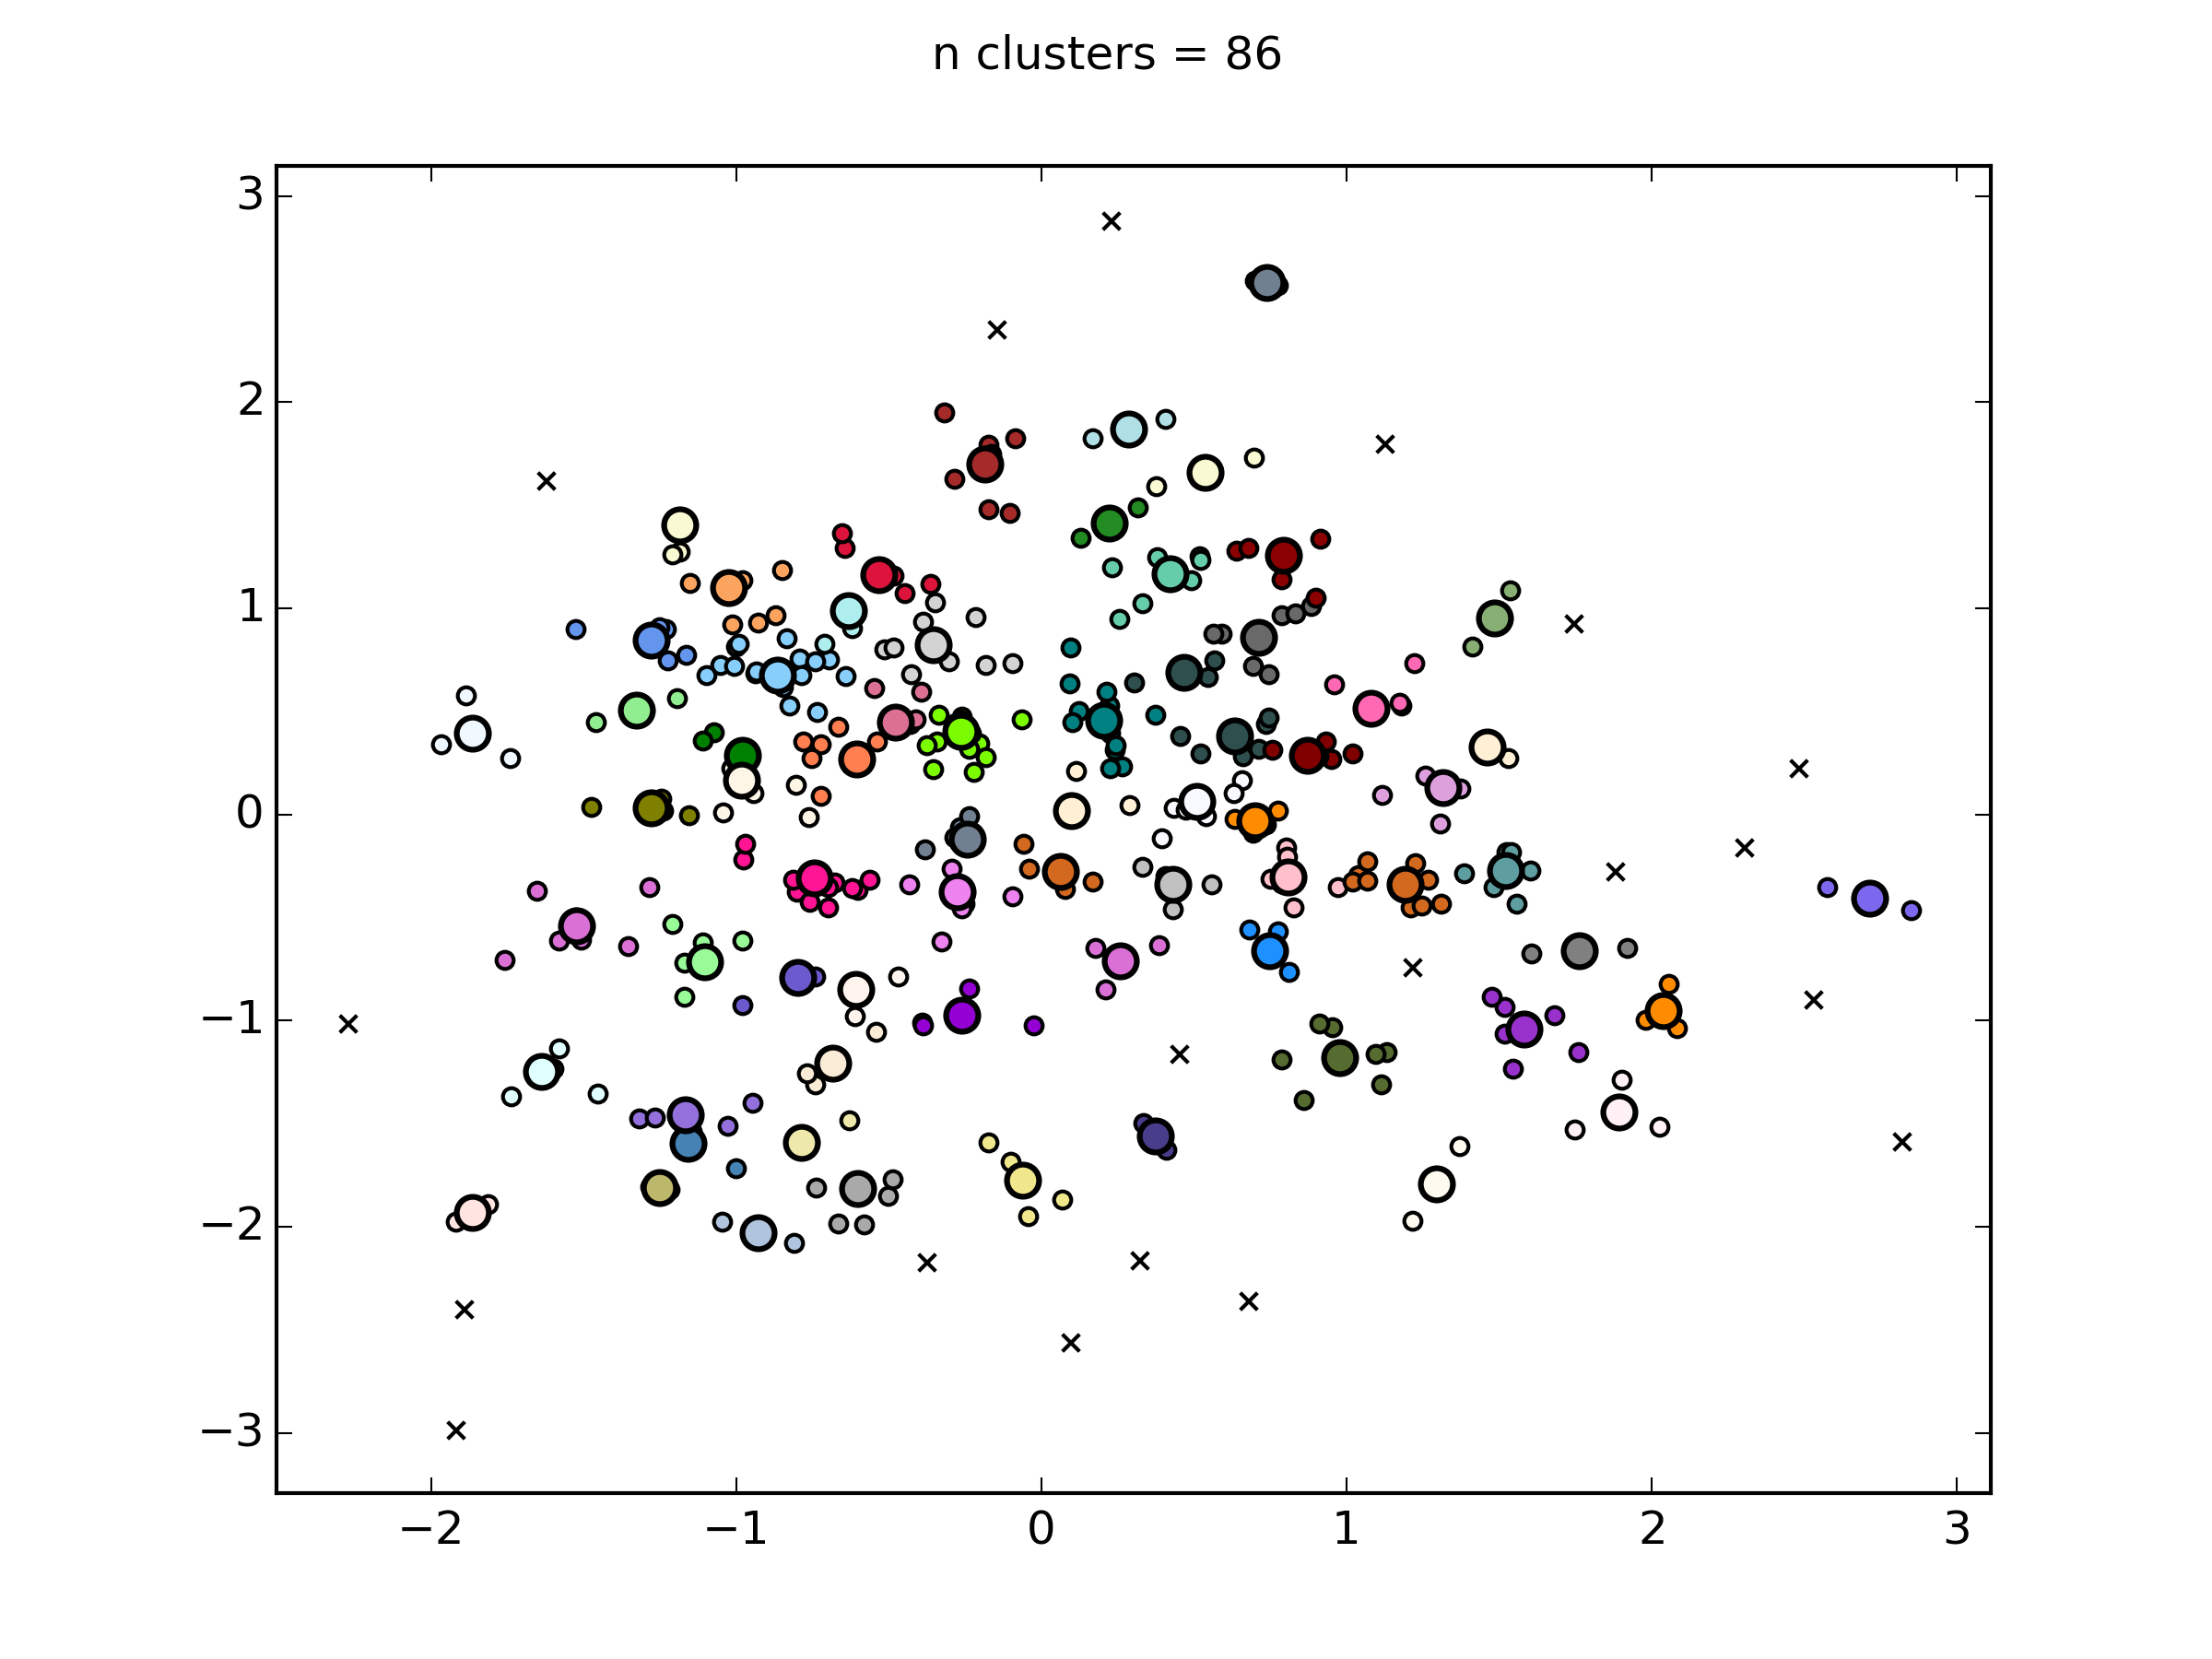
\includegraphics[width=0.9\textwidth]{birch_clustering.png}
      \caption{"BIRCH clustering of a single day"}
      \label{birch_clustering}
  \end{figure}

The second approach with the BIRCH algorithm, yielded some interesting results as well. We can see in figure \ref{birch_clustering}, that there are a lot of clusters of different sizes.
In news events, we mainly want smaller coherent clusters. The centroids are the bigger points painted in a distinct color. Smaller points are documents, assigned to a centroid in the same color. Further, the scaling of the displayed points is normalized by average on a coincidence matrix projected down by \lsa{} and \pca{}.\\

The data at hand does not stem from the BBC data set, but from daily scraped newspapers. The papers shall not be named due to legal reasons. One can see, that the resulting clusters are small and well formed. Some cluster centers are bigger than others. In those cases, we can recluster them to further enhance the variance of clusters. The structures resemble, that there are news that are covered several times a day and some that are not. Singleton clusters are presented as $x$, for one time events. Those outliers can be reclustered in a different run and would cover news like ``other''.

  \begin{figure}[h!]
    \centering
      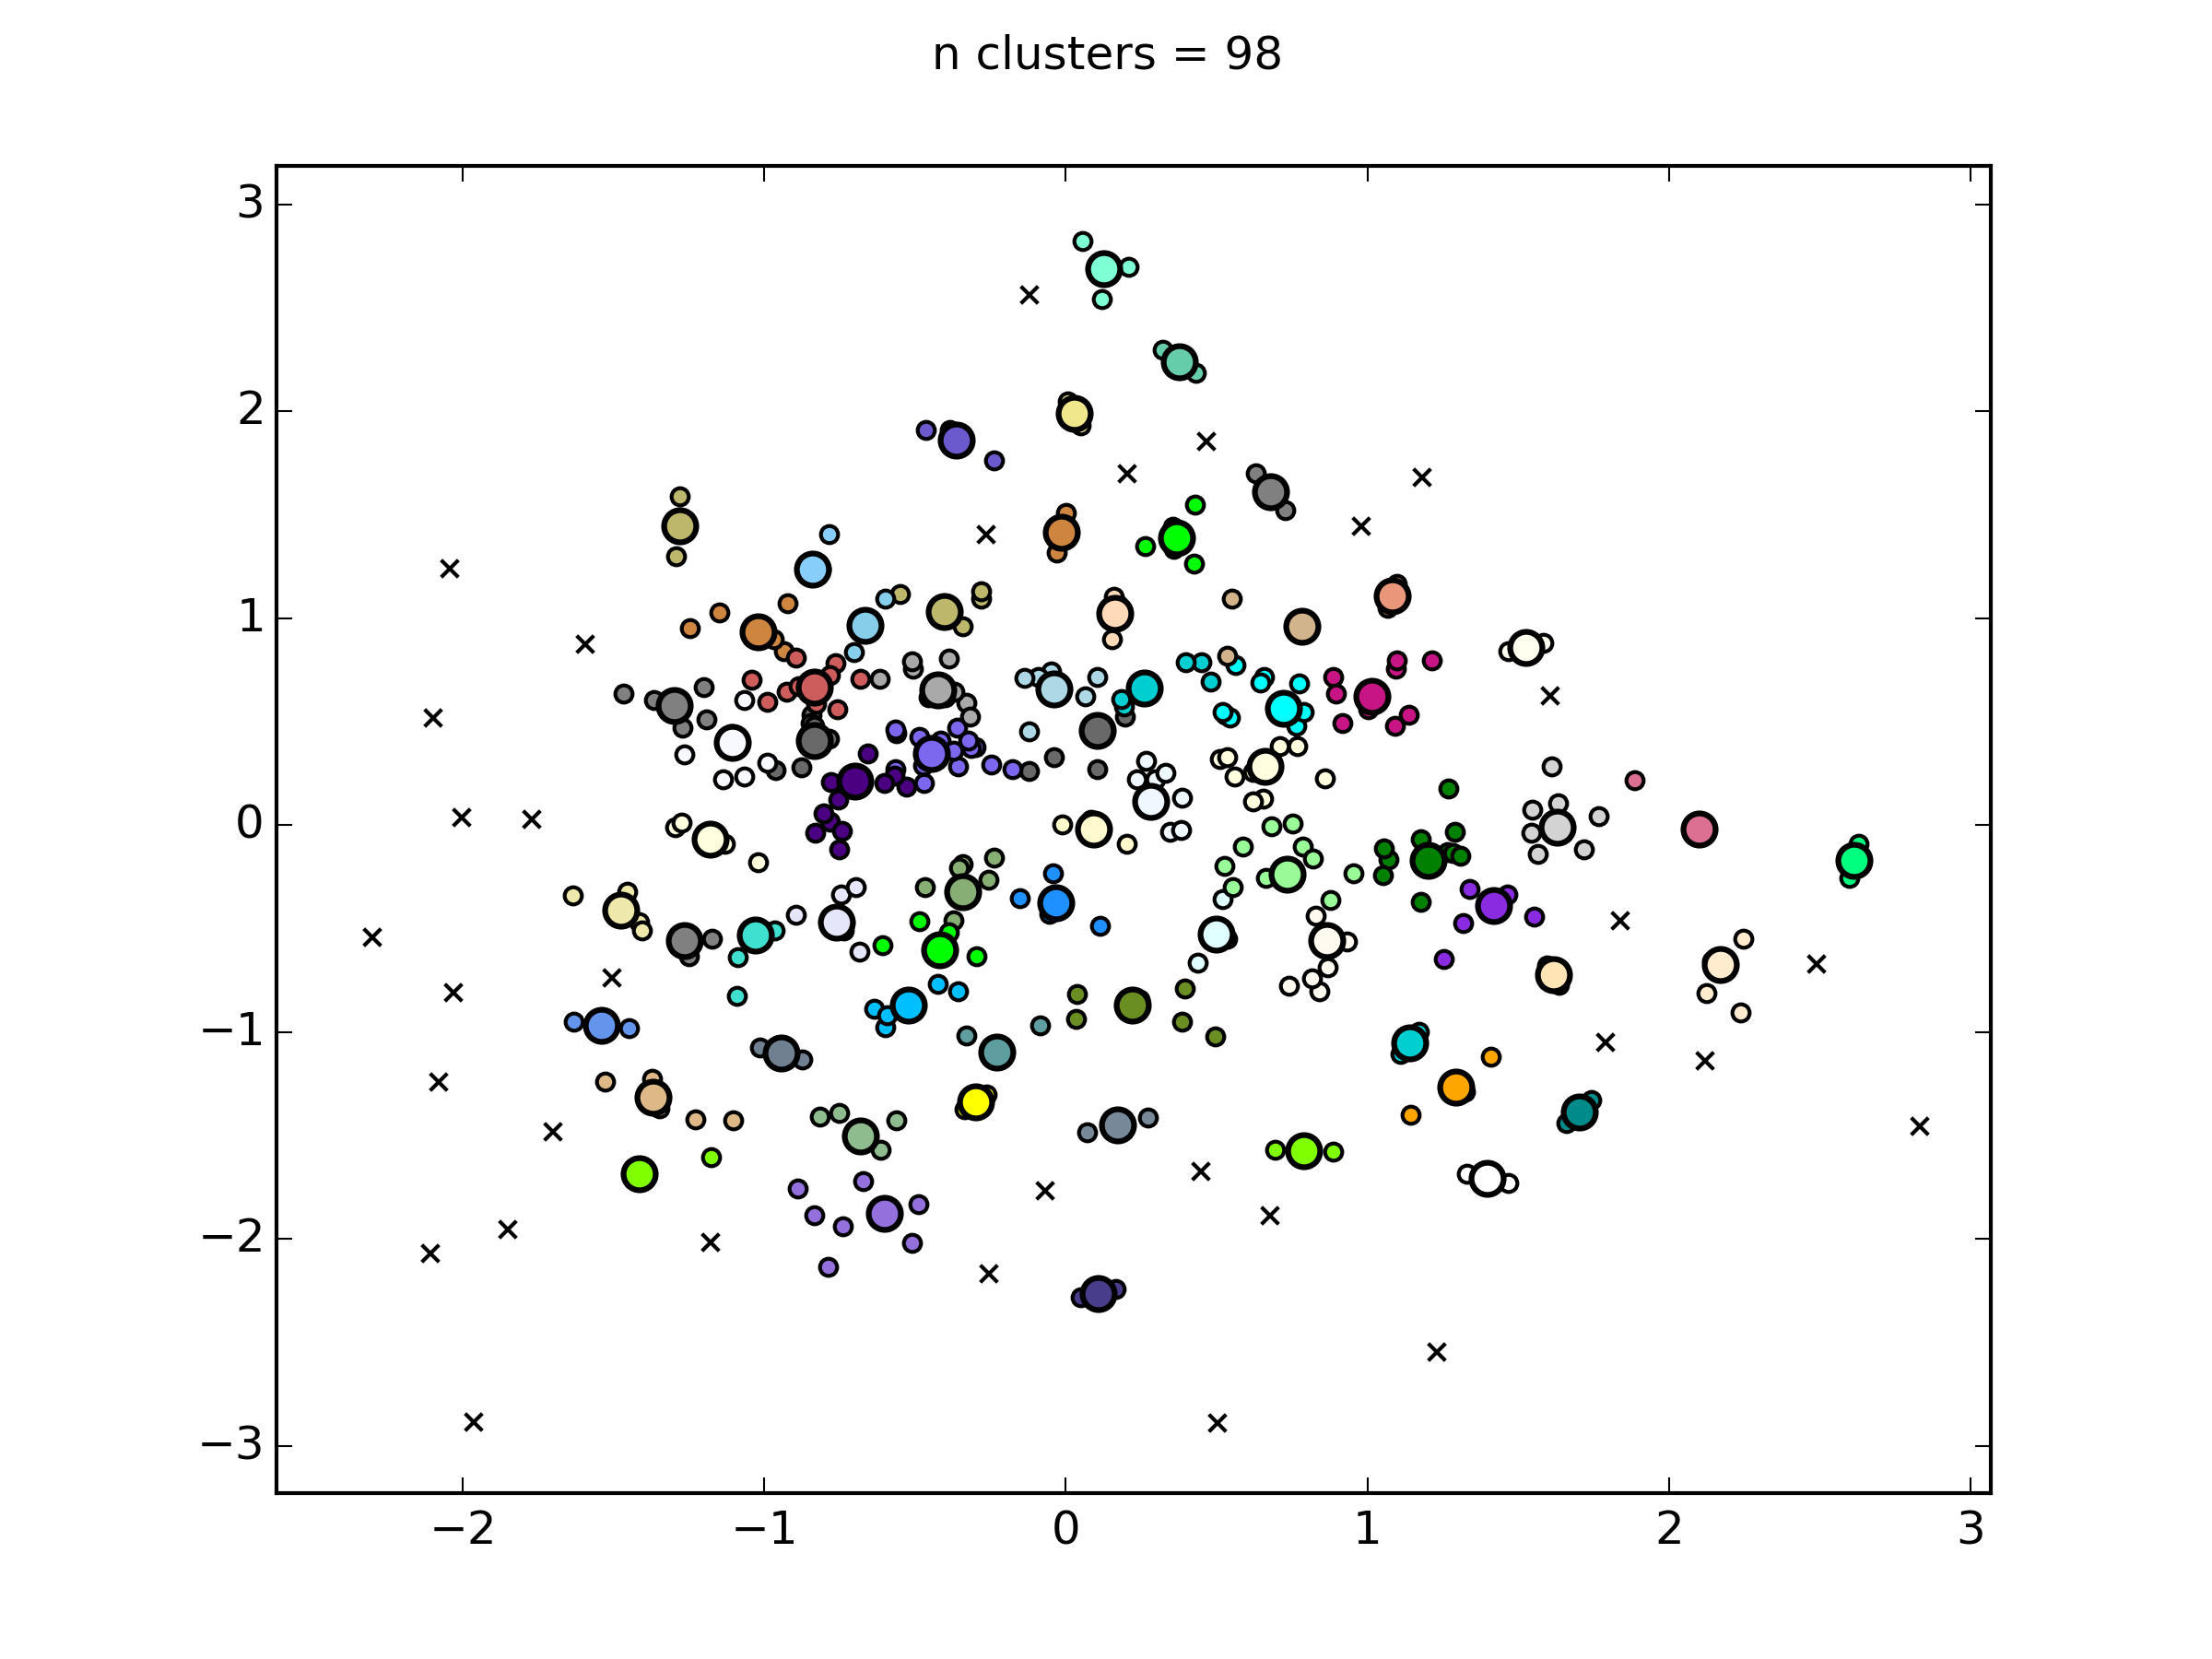
\includegraphics[width=0.9\textwidth]{mean_shift_clustering.png}
      \caption{"Mean Shift clustering of a single day"}
      \label{mean_shift_clustering}
  \end{figure} 

Figure \ref{mean_shift_clustering} is a clustering with the \emph{Mean Shift} algorithm. It is a partitonal algorithm working with density distributions, automatically inferring the size of clusters by threshold. The clusters of the \emph{Mean Shift} are smaller and the density threshold was carefully fine tuned.\\ 

All visualizations were made of data containing roughly 350 documents from the category \emph{world} by two newspapers. Expecting at least 100 events covering different news. The final clustering visualizations are a result of several parameter estimations of the algorithms. All visualizations were done with the help of a Python API called \emph{matplotlib} by \cite{MatPlotHunter2007}.

\section{Multiple days clustering}
  Multiple days clustering was of the greatest interest while starting this thesis. It came to an understanding, that it is inherently difficult to cluster and track documents over the course of several weeks. The time ran out to actually cluster multiple days in a row. Also, due to the problem of legality, the BBC data set came to the rescue. Multiple days clustering is an advancement on the single day clustering. See section \ref{sec:future_work} for future work on this matter.



